\section{Movimiento oscilatorio}
  \subsection{Movimiento de un objeto unido a un resorte}
    \PN \textit{Posición de equilibrio}: Cuando el resorte no está estirado ni comprimido el bloque queda en reposo.

    \vspace{3mm}
    \PN Consideremos el siguiente modelo:

    \begin{figure}[H]
    \centering
      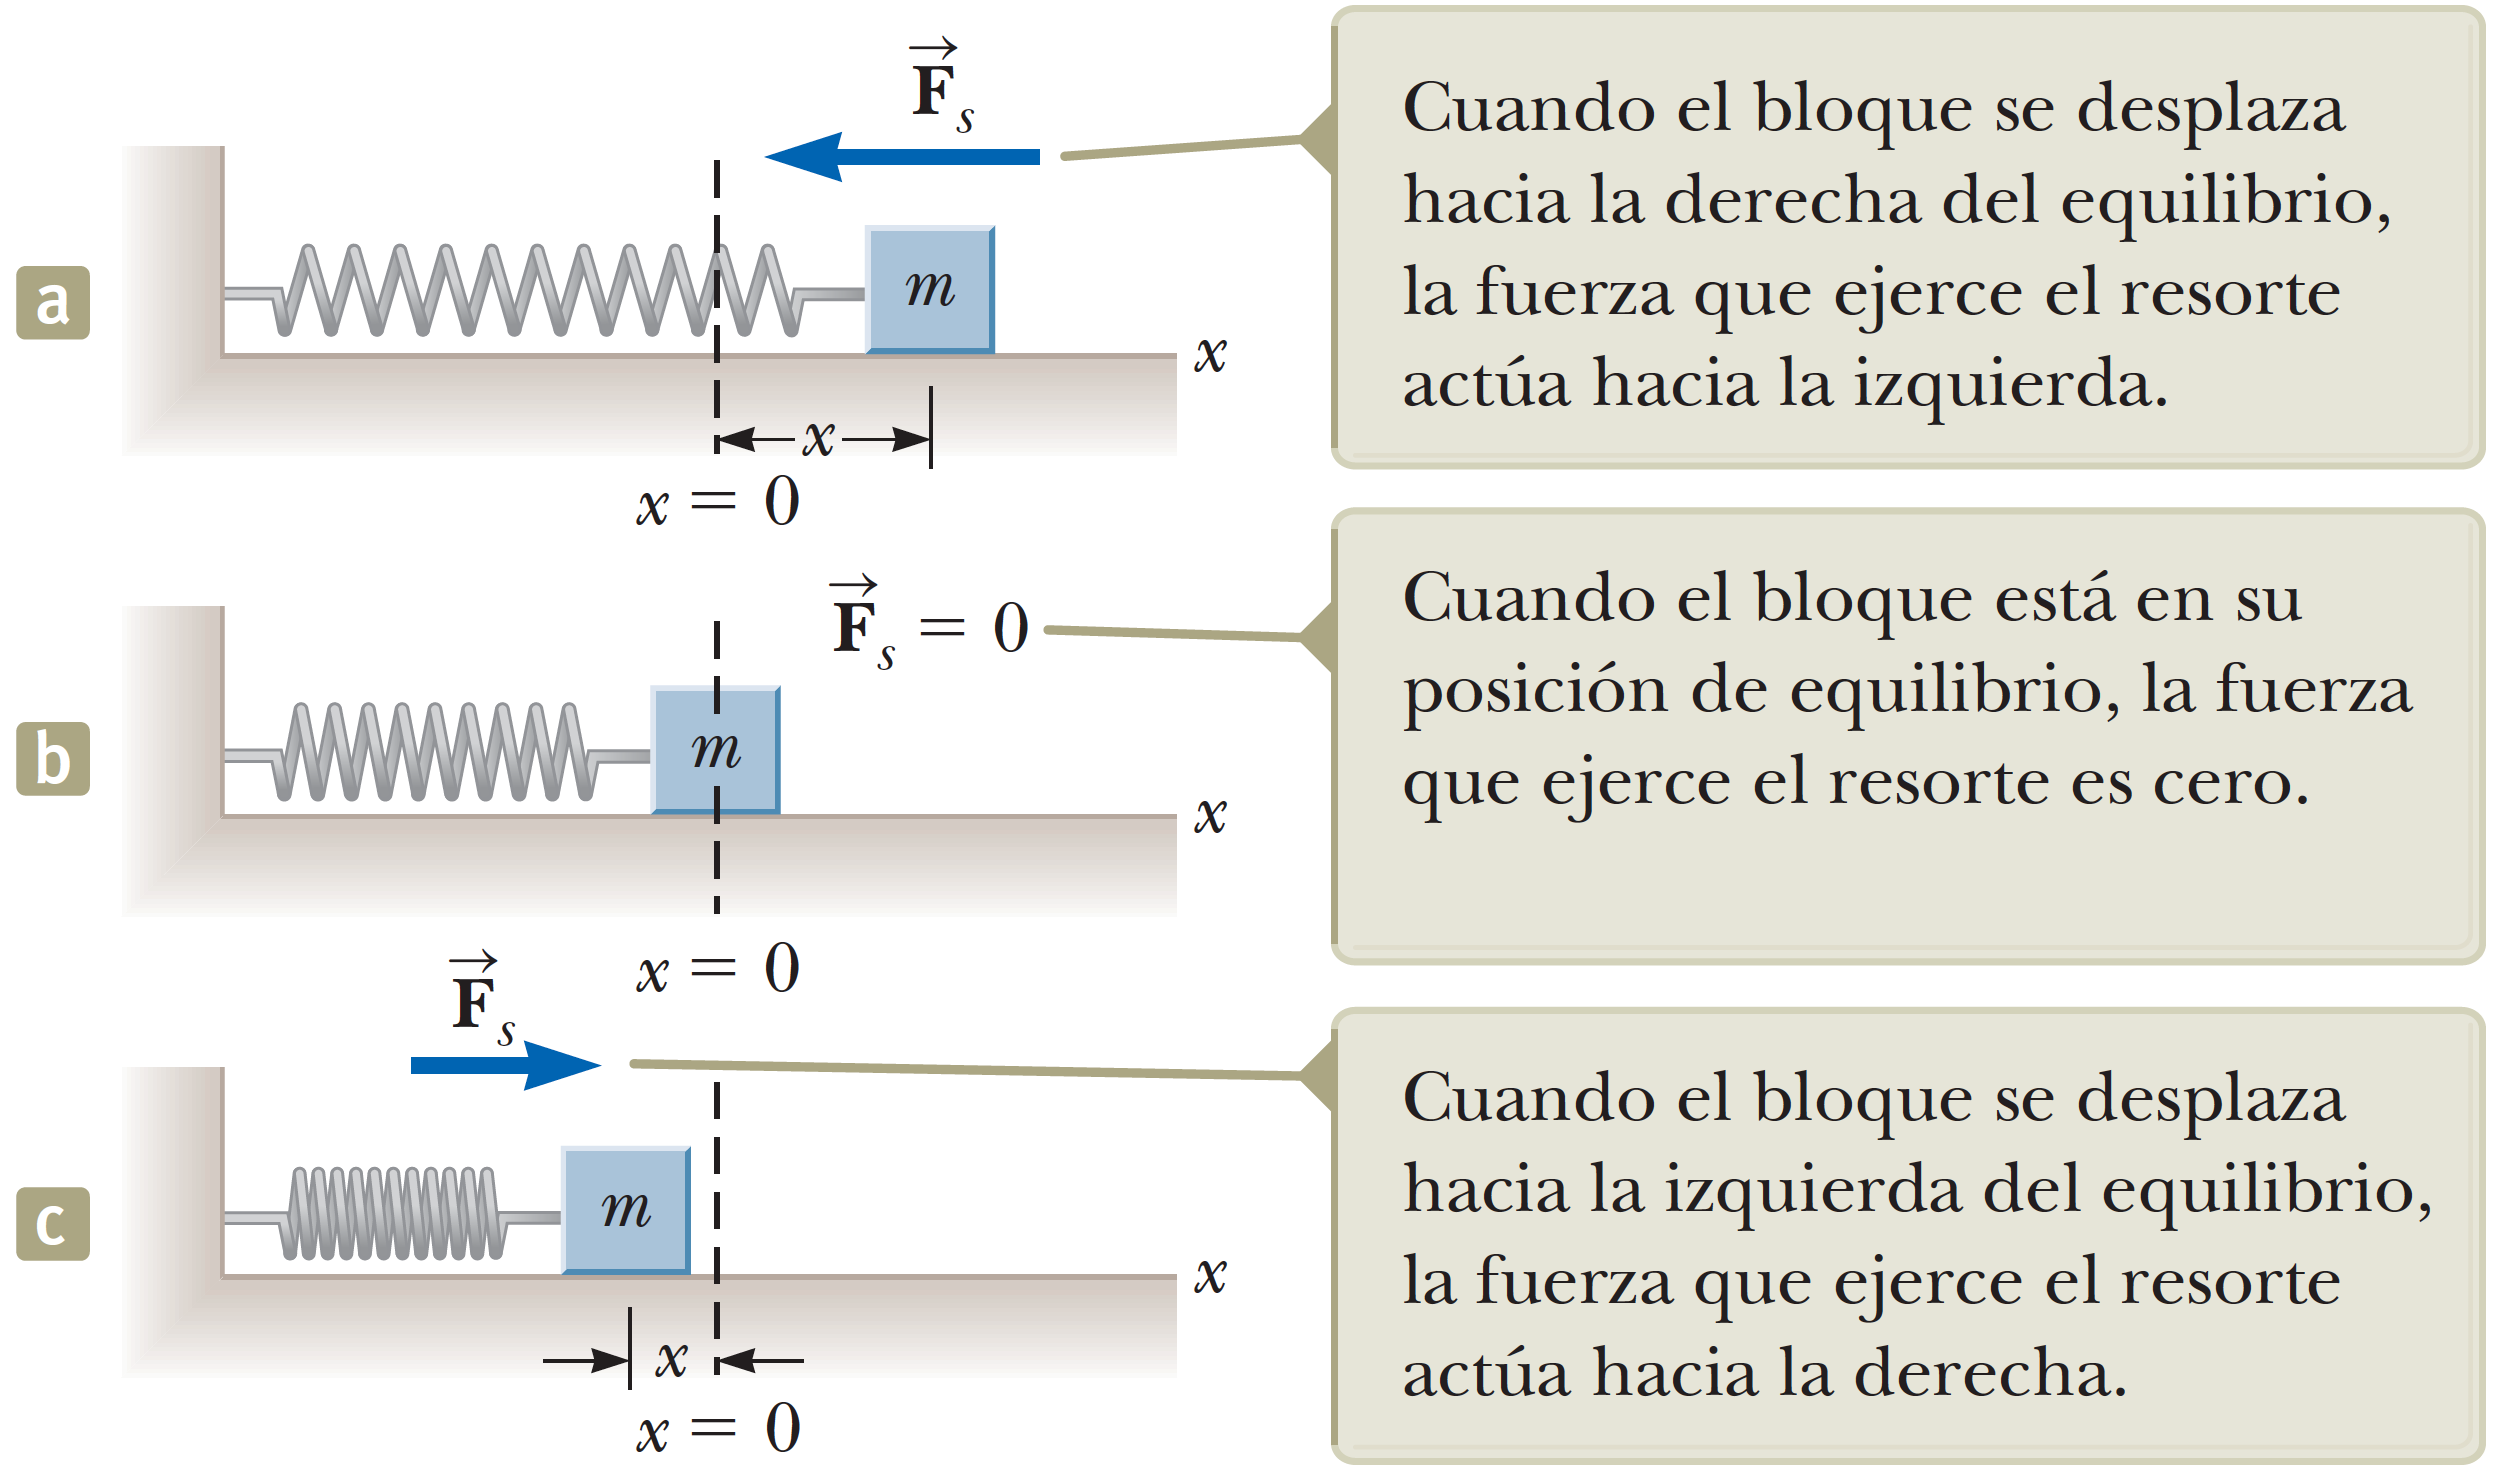
\includegraphics[width=0.6\textwidth]{2/figure_1}
      \caption{Bloque unido a un resorte móvil sobre una superficie sin fricción.}
    \end{figure}

    \PN Cuando el bloque se desplaza a una posición x, el resorte ejerce sobre el bloque una fuerza que es proporcional a
    la posición y está dada por la \textbf{ley de Hooke}:
    \begin{equation}\label{eq:1}
      \underbrace{F_{s}}_{\text{fuerza restauradora}} = -\underbrace{k}_{\text{constante elástica}}\underbrace{x}_{\text{compresión}}
    \end{equation}
    \PN Cuando el bloque es desplazado desde el punto de equilibrio y se suelta, éste es una partícula bajo una fuerza
    neta y, en consecuencia, experimenta una aceleración. Al aplicar la segunda ley de Newton al movimiento del bloque,
    con la ecuación \ref{eq:1} que proporciona la fuerza neta en la dirección x, se obtiene:
    \begin{eqnarray*}
      \Sigma \ F_{x} = ma_{x} &\rightarrow& -kx = ma_{x} \\
      a_{x} &=& \frac{-k}{m}x
    \end{eqnarray*}

    \PN Se dice que los sistemas en los cuales la aceleración del bloque es proporcional a su posición, y la dirección de
    la aceleración es opuesta a la dirección del desplazamiento del bloque desde el equilibrio exhiben \textbf{movimiento
    armónico simple}.

    \PN En ausencia de fricción este movimiento idealizado continuará por siempre porque la fuerza que ejerce el resorte
    es conservativa.

  \subsection{Partícula en movimiento armónico simple}
    \PN La posición de un objeto actuando sobre una fuerza descrita por la \textit{Ley de Hooke} esta dada por:
    \begin{equation}
      x(t) = A \cos (\omega t)
    \end{equation}

    \PN donde A, $\omega$, son constantes y:
    \begin{itemize}
      \item Amplitud del movimiento (A): es simplemente el máximo valor de la posición de la partícula en la dirección x
      positiva o negativa.
      \item Frecuencia angular ($\omega$): es una medida de qué tan rápido se presentan las oscilaciones;
      mientras más oscilaciones por unidad de tiempo haya, más alto es el valor.
      \begin{equation}
        \omega = \sqrt{\frac{k}{m}}
      \end{equation}
      \item Período del movimiento (T): es el intervalo de tiempo requerido para que la partícula pase a través de un
      ciclo completo de su movimiento.
      \begin{equation}
        T = \frac{2\pi}{\omega} = 2\pi \sqrt{\frac{m}{k}}
      \end{equation}
      \item Frecuencia (f): representa el número de oscilaciones que experimenta la partícula por unidad de intervalo de
      tiempo.
      \begin{equation}
        f = \frac{1}{T} = \frac{1}{2\pi} \sqrt{\frac{k}{m}}
      \end{equation}
    \end{itemize}

    \PN \textbf{Ecuaciones de velocidad y de aceleración}
    \begin{eqnarray*}
      v = \frac{dx}{dt} &=& - \omega A \sin (\omega t) \\
      a = \frac{d^{2}x}{dt^{2}} &=& - \omega^{2} A \cos (\omega t)
    \end{eqnarray*}

    \PN \textbf{Valores máximos}
    \begin{eqnarray*}
      x_{max} &=& A \\
      v_{max} &=& \omega A = \sqrt{\frac{k}{m}} \\
      a_{max} &=& \omega^{2} A = \frac{k}{m} A
    \end{eqnarray*}

  \subsection{Energía del oscilador armónico simple}
    \PN \textbf{Energía cinética}
    \begin{equation}
      K = \frac{1}{2} m v^{2} = \frac{1}{2} m \omega^{2} A^{2} \sin^{2} (\omega t)
    \end{equation}

    \PN \textbf{Energía potencial}
    \begin{equation}
      U = \frac{1}{2} k x^{2} = \frac{1}{2} k A^{2} \cos^{2} (\omega t)
    \end{equation}

    \PN \textbf{Energía total}
    \PN Dado que K y U siempre son cantidades positivas o cero. Puesto que $\omega^{2} = \frac{k}{m}$, la energía mecánica
    total del oscilador armónico simple se expresa como:
    \begin{eqnarray*}
      E &=& K + U = \frac{1}{2} k A^{2} [\sin^{2} (\omega t) + \cos^{2} (\omega t)] \\
      &=& \frac{1}{2} k A^{2}
    \end{eqnarray*}

    \pagebreak
    \PN \textbf{Velocidad como una función de la posición}
    \PN La velocidad del bloque en una posición arbitraria se obtiene al expresar la energía total del sistema en alguna
    posición arbitraria x como:
    \begin{eqnarray*}
      E &=& K + U = \frac{1}{2} m v^{2} + \frac{1}{2} k x^{2} = \frac{1}{2} k A^{2} \\
      v &=& \pm \sqrt{\frac{k}{m} (A^{2} - x^{2})} = \pm \omega \sqrt{A^{2} - x^{2}}
    \end{eqnarray*}

  \subsection{Osciladores amortiguados}
    \PN En muchos sistemas reales, fuerzas no conservativas como la fricción o la resistencia del aire retardan el
    movimiento del sistema. En consecuencia, la energía mecánica del sistema disminuye en el tiempo y se dice que el
    movimiento está amortiguado.

    \vspace{3mm}
    \PN Consideremos el siguiente modelo:

    \begin{figure}[H]
    \centering
      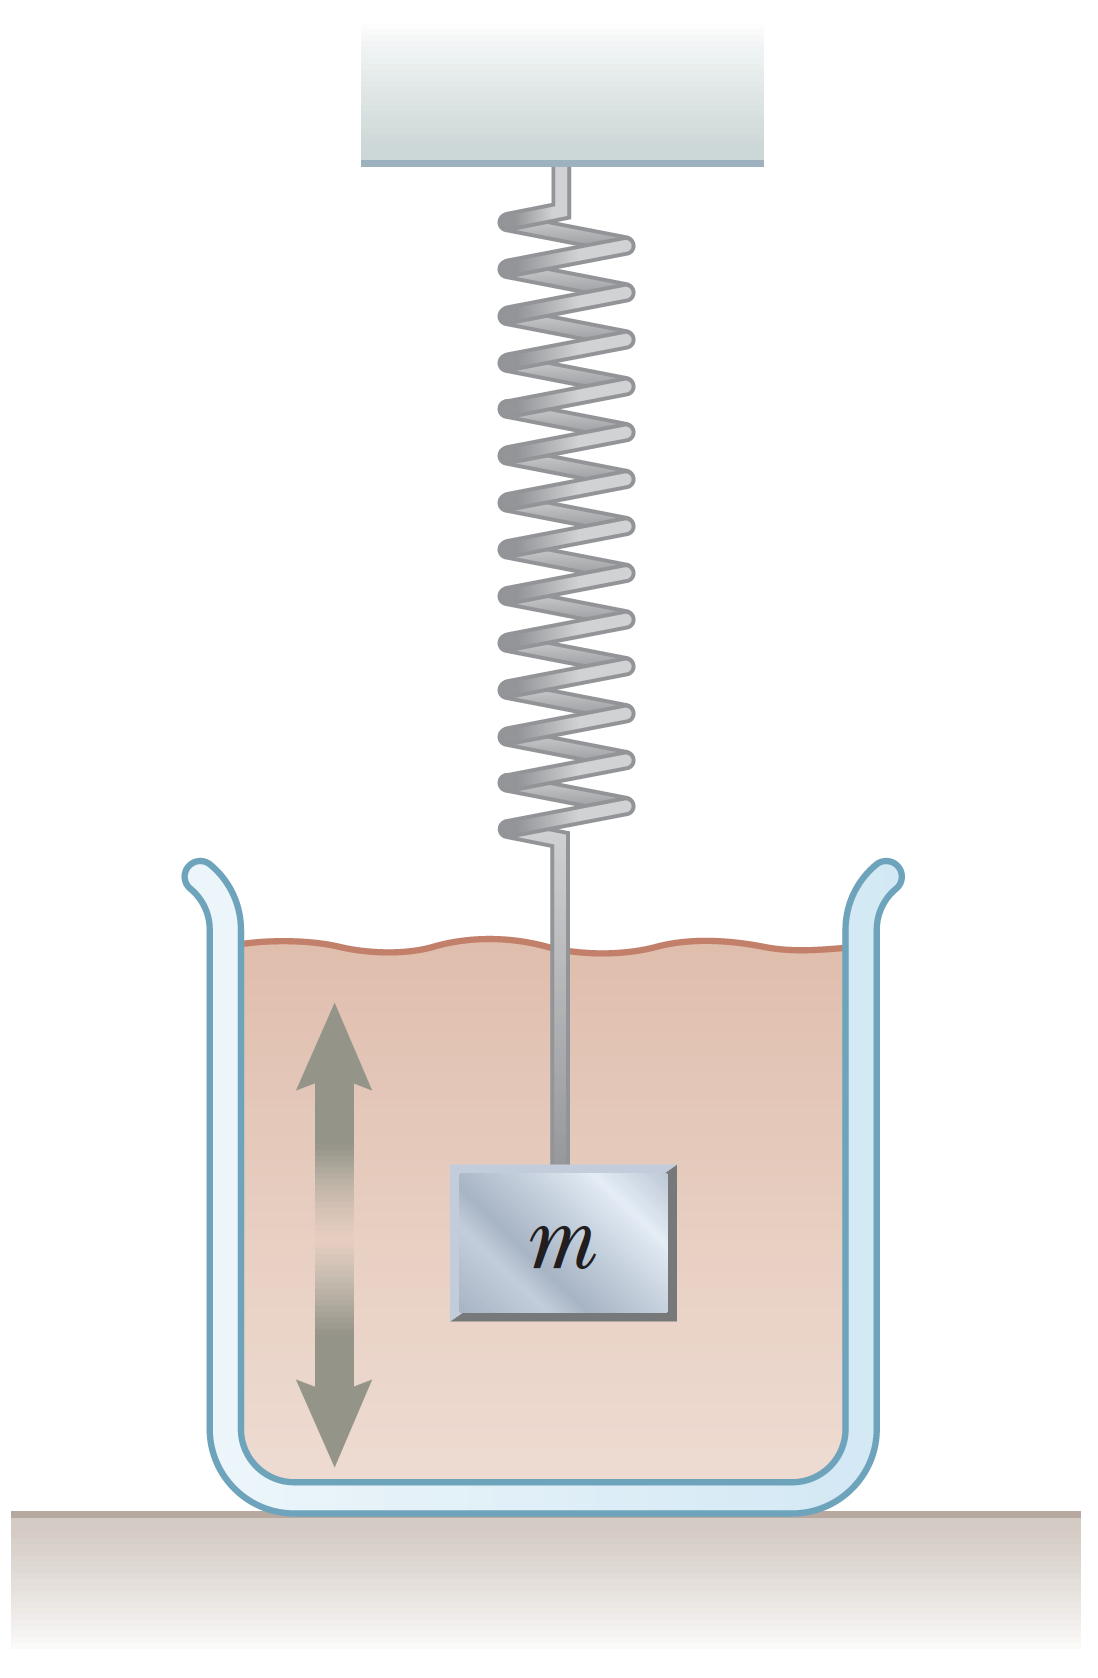
\includegraphics[width=0.15\textwidth]{2/figure_2}
      \caption{Ejemplo de un oscilador amortiguado es un objeto unido a un resorte y sumergido en un líquido viscoso.}
    \end{figure}

    \PN Se puede escribir la segunda ley de Newton como:
    \begin{eqnarray*}
      \Sigma \ F_{x} &=& -kx - \underbrace{b \overbrace{v}^{\text{coeficiente de amortiguamiento}}}_{\text{fuerza retardadora}} = ma_{x} \\
      -kx - b \frac{dx}{dt} &=& m \frac{d^{2}x}{dt^{2}}
    \end{eqnarray*}

    \PN \textbf{Ecuación de la posición}
    \begin{equation}
      x(t) = A \mathrm{e}^{\frac{-b}{2m}t} \cos (\omega t)
    \end{equation}

    \PN donde la frecuencia angular de oscilación es:
    \begin{equation}
      \omega = \sqrt{\frac{k}{m} - \left(\frac{b}{2m}\right)^{2}}
    \end{equation}

    \PN Es conveniente expresar la frecuencia angular de un oscilador amortiguado en la forma:
    \begin{equation}
      \omega = \sqrt{\omega_{0} - \left(\frac{b}{2m}\right)^{2}}
    \end{equation}

    \PN donde $\omega_{0} = \sqrt{k/m}$ representa la frecuencia angular en ausencia de una fuerza retardadora (el
    oscilador no amortiguado) y se llama \textbf{frecuencia natural} del sistema.

    \pagebreak
    \PN \textbf{Tipos de amortiguamiento}
    \begin{itemize}
      \item Subamortiguado: $\omega_{0} > \frac{b}{2m}$
      \item Críticamente Amortiguado: $\omega_{0} = \frac{b}{2m}$
      \item Sobreamortiguado: $\omega_{0} < \frac{b}{2m}$
    \end{itemize}

  \subsection{Oscilaciones forzadas}
    \PN Se ha visto que la energía mecánica de un oscilador amortiguado disminuye en el tiempo como resultado de la fuerza
    retardadora. Es posible compensar esta disminución de energía al aplicar una fuerza externa que haga trabajo positivo
    sobre el  sistema. En cualquier instante se puede transferir energía al sistema mediante una fuerza aplicada que actúe
    en la dirección de movimiento del oscilador.

    \PN Al modelar un oscilador con fuerzas retardadoras e impulsoras como una partícula bajo una fuerza neta, la segunda
    ley de Newton en esta situación produce:
    \begin{equation}
      \Sigma \ F_{x} = ma_{x} \rightarrow F_{0} \sin (\omega t) -b \frac{dx}{dt} - kx = m \frac{d^{2}x}{dt^{2}}
    \end{equation}

    \PN \textbf{Ecuación de la posición}
    \begin{equation}
      x(t) = A \cos (\omega t)
    \end{equation}

    \PN donde
    \begin{equation}
      A = \frac{F_{0}/m}{\sqrt{\left(\omega^{2} - \omega_{0}^{2}\right)^{2} - \left(\frac{b\omega}{m}\right)^{2}}}
    \end{equation}

    \PN y donde $\omega_{0} = \sqrt{k/m}$ es la frecuencia natural del oscilador subamortiguado ($b = 0$).
